\subsection{The \macro{CORRESP}}\label{sec:ca-camacro}

The steps illustrated in \exref{ex:haireye3} are not difficult, but it is somewhat tedious to do them repeatedly.
The \macro{CORRESP} (documented in \macref{mac:corresp})
is designed to make it easy to produce reasonable plots for \CA\
results.

The \macro{CORRESP}
\begin{itemize}
\item is designed as a simple macro interface to the \proc{CORRESP}.

\item It handles input in either contingency table form
(columns specified by the \mparm{VAR=}{CORRESP}, rows by the
\mparm{ID=}{CORRESP}), or frequency or case form 
(using the \mparm{TABLES=}{CORRESP}).

\item Three-way and larger tables may be analyzed by the ``stacking''
approach to
\mway\ tables described in \secref{sec:ca-multiway}, or by
the MCA approach.

\item Optionally, the macro produces a labeled printer plot and/or
\hires\ graphics plot, with many options for controlling the appearance
of graphics plots.
Axes for \hires\ plots may be equated automatically.
\item An \ODS\ containing the point coordinates and an \ADS\ containing point labels
are produced for further plotting or customization.
\end{itemize}

\begin{Example}[mental1]{Mental impairment and parents' SES}
\citet[p. 289]{Srole-etal:78} give the data below on the mental
health status of a sample of 1660 young New York residents in midtown Manhattan
classified by their parents' socioeconomic status (SES);
see \datref{dat:mental}.
There are five categories of SES and mental health is classified
in the four categories ``well'', ``mild symptom formation'',
``moderate symptom formation'', and ``impaired''.
These data have also been analyzed by many authors, including
\citet[ \S 8.5.2]{Agresti:90},
\citet{Goodman:79}, and
\citet[p. 375]{Haberman:79}.

The statements below read the data in contingency table form with rows identified
by the variable \pname{SES} and column variables \pname{well mild moderate impaired}.
These variables are used in the \verb|%CORRESP| call as the \pname{ID=}
and \pname{VAR=} parameters, respectively.
The graphics output is shown in \figref{fig:correses}.
\begin{figure}[htb]
  \centering
  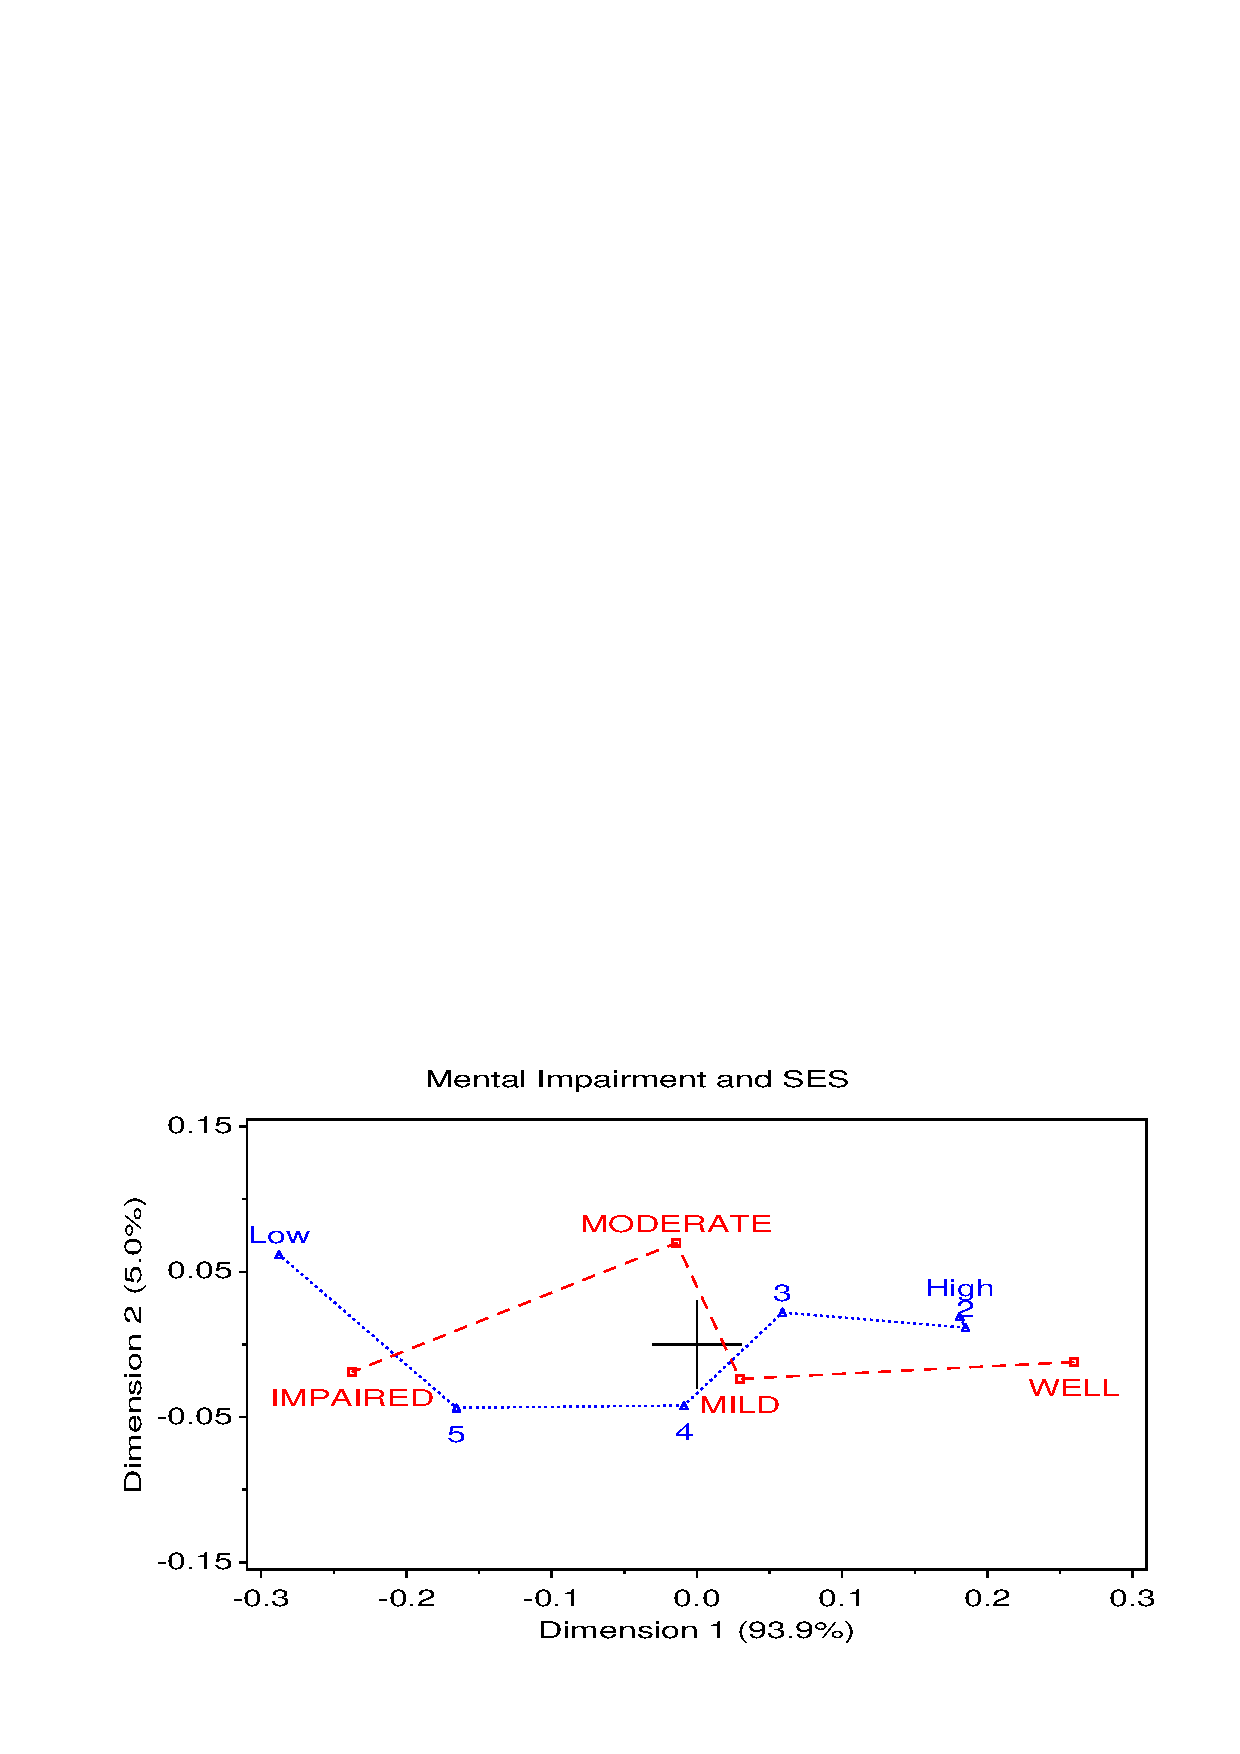
\includegraphics[scale=.8,clip=true]{ch\thechapter/fig/correses}
  \caption{\macro{CORRESP} plot for Mental Health data}\label{fig:correses}
\end{figure}
%% input: /Users/friendly/sasuser/catdata/correses.sas
%% last modified: 25-Jul-99  8:31
\begin{listing}
title h=1.5 lspace=3.8in 'Mental Impairment and SES';
data mental;
   input ses $ well mild moderate impaired;
datalines;
High 64     94     58     46
2    57     94     54     40
3    57    105     65     60
4    72    141     77     94
5    36     97     54     78
Low  21     71     54     71
;
axis1 length=3 in  order=(-.15 to .15 by .10)
      label=(h=1.5 a=90 r=0);
axis2 length=6 in  order=(-.30 to .30 by .10)
      label=(h=1.5) offset=(1);
%corresp (data=mental, id=ses, var=Well Mild Moderate Impaired,
      vaxis=axis1, haxis=axis2, htext=1.3, pos=-, interp=join,
      symbols=triangle square);
\end{listing}

Some of the graphics options for the \macro{CORRESP}
are illustrated by the \pname{htext=} (height of text labels),
\pname{pos=} (position of text labels), \pname{interp=} (point marker interpolation),
and \pname{symbols=} (point symbols) options.
In particular, the option \pname{pos=-} causes the macro to position the text labels
centered above or below the point depending on whether the $y$ position is positive
or negative
(as provided by the \macro{LABEL}; see \macref{mac:label}).

The cross at the origin in \figref{fig:correses} is drawn with equal data units in the
$x$ and $y$ direction, and so serves as a guide to whether the axes
have been equated.  The \pname{LENGTH} and \pname{ORDER} values on the \stmt{AXIS}{GPLOT}s
shown above
were determined by inspection after an initial plot.

We see from the plot that the association between mental health
and parents' SES is almost entirely 1-dimensional, with 94\% of
the \chisq\ ( 45.98, with 15 df) accounted for by Dimension 1.
The diagnostic categories are well-aligned with this dimension and
the two intermediate categories are closer on this dimension than
the extremes, indicating that their profiles differ little.  The
SES categories are also aligned with Dimension 1, and approximately
equally spaced, with the exception of the highest two categories.
Because both row and column categories have the same pattern on
Dimension 1, we may interpret the plot as showing that the profiles
of both variables are ordered, and their relation can be explained
as a positive association between parents' SES and higher mental
health status of children.

From a modeling perspective,  we might ask how strong is the evidence
for the spacing of categories noted above.  For example, we might
ask whether assigning integer scores to the levels of SES and mental
impairment provides a simpler, but satisfactory account of their association.
This question will be explored in a later chapter (see \exref{ex:mental2}).
\end{Example}
